%%%%%%%%%%
% [TODO] %
%%%%%%%%%%
% [ ] Better figures for the annexes 
% [ ] Add correlation ABX-id
% [ ] Figure captions

%%%%%%%%%%%%%%%%%%%%%%
% Chapter mini-intro %
%%%%%%%%%%%%%%%%%%%%%%

%% Short background %%

[Short BG] \\

%% Research questions (+ alternatives) %%

[Research questions] \\

%% Plan %%

In \textbf{section 2.1} a perceptual experiment aims to disentangle the contributions of phonetic categories and acoustic details on epenthetic vowel quality. Participants are asked to report their choice of epenthetic vowel (if any) within consonant cluster in stimuli where the acoustic information contained in the cluster may be in disagreement with the identity of neighbouring vowels. Information theoretic measures allow to quantify the influence of both neighbouring phonetic categories and acoustic details.  


In \textbf{section 2.2} I investigate the possibility of predicting epenthetic vowel quality in Brazilian Portuguese (BP) and Japanese (JP) using a production-based exemplar model of perception. This type of model predicts the quality of a vowel epenthesized within the cluster of a stimulus based solely on the acoustic similarity of said /CC/ cluster to /CVC/ exemplars produced by native speakers of BP or JP. From this modelling approach we can evaluate the influence of pure acoustics on effects such as default epenthetic vowel quality and modulations induced by neighbouring vowels.

%%%%%%%%%%%%%%%%%%%%
% /ahpa/ (JASA-EL) %
%%%%%%%%%%%%%%%%%%%%

%%%% Main %%%%
\includepdf[pages={2-8}, pagecommand={},
addtotoc={
  2,section,1,Which epenthetic vowel? \\ Phonetic categories versus acoustic detail in perceptual vowel epenthesis,ahpa_main,
  3,subsection,2,Methods,ahpa_methods,
  4,subsection,2,Results,ahpa_results,
  6,subsection,2,Discussion,ahpa_disc,
  7,subsection,2,References,ahpa_ref}]
{images/chapter02/JASAEL_Guevara-Rukoz_2017_Which_epenthetic_vowel.pdf}

%%%% Annexes %%%%
\subsection{Annexes}

\subsubsection{Acoustic analyses}
\begin{figure}[H]
  \centering
  \begin{overpic}[page=1, width=0.8\linewidth]{chapter02/ahpa_acoustic}\end{overpic}
  \caption{Figure caption}
  \label{fig:ahpa_acoustic}
\end{figure}

\subsubsection{Control items}
\begin{figure}[H]
  \centering
  \begin{overpic}[page=1, width=0.2\linewidth]{chapter02/ahpa_uep-copyep}\end{overpic}
  \hspace{2cm}
  \begin{overpic}[page=2, width=0.2\linewidth]{chapter02/ahpa_uep-copyep}\end{overpic}
  \caption{Figure caption}
  \label{fig:ahpa_uep-copyep}
\end{figure}

\subsubsection{Test items (by speaker)}
\begin{figure}[H]
  \centering
  \begin{overpic}[page=1, width=\linewidth]{chapter02/ahpa_heath_spk}\end{overpic}
  \caption{Figure caption}
  \label{fig:ahpa_spk}
\end{figure}

\subsubsection{ABX task}
% [TODO] Add correlation results
We also performed a control ABX task with a different set of participants, as this task promotes a more global perception of the stimuli. In this experiment, participants heard trials with 4 types of AB pairs:
\begin{itemize}
    \item $V_1CpV_1$ (non-spliced cluster) vs. $V_1CV_1pV_1$ (full vowel)
    \item $V_1CpV_1$ (non-spliced cluster) vs. $V_1C_{V_2}pV_1$ (spliced cluster)
    \item $V_1C_{V_2}pV_1$ (spliced cluster) vs. $V_1C_{V_3}pV_1$ (spliced cluster)
    \item $V_1C_{V_2}pV_1$ (spliced cluster) vs. $V_1CV_2pV_1$ (full vowel)
\end{itemize}

\begin{figure}[H]
  \centering
  \begin{overpic}[page=6, width=0.9\linewidth]{chapter02/ahpa_figs}\end{overpic}
  \caption{Figure caption}
  \label{fig:ahpa_abx}
\end{figure}

We saw that ABX accuracy rates for each pair were correlated with how similar response patterns for items A and B were at the identification task. In other words, the more similar response patterns were for A and B at the identification task, the harder it was for participants to discriminate A and B at the ABX task. \\

Similarity of responses was assessed by computing the Euclidean distance between 6-dimensional vectors [$p_{none}$, $p_a$, $p_e$, $p_i$, $p_o$, $p_u$] of A and B, where $p_x$ corresponds to the proportion of total trials for A (or B) in which participants responded $x$. These results suggest that adaptation patterns attested in the identification task are not task-dependent.


%%%%%%%%%%%%%%%%%%%%%%%%%%
% Parlato1 (Interspeech) %
%%%%%%%%%%%%%%%%%%%%%%%%%%

%%%% Main %%%%
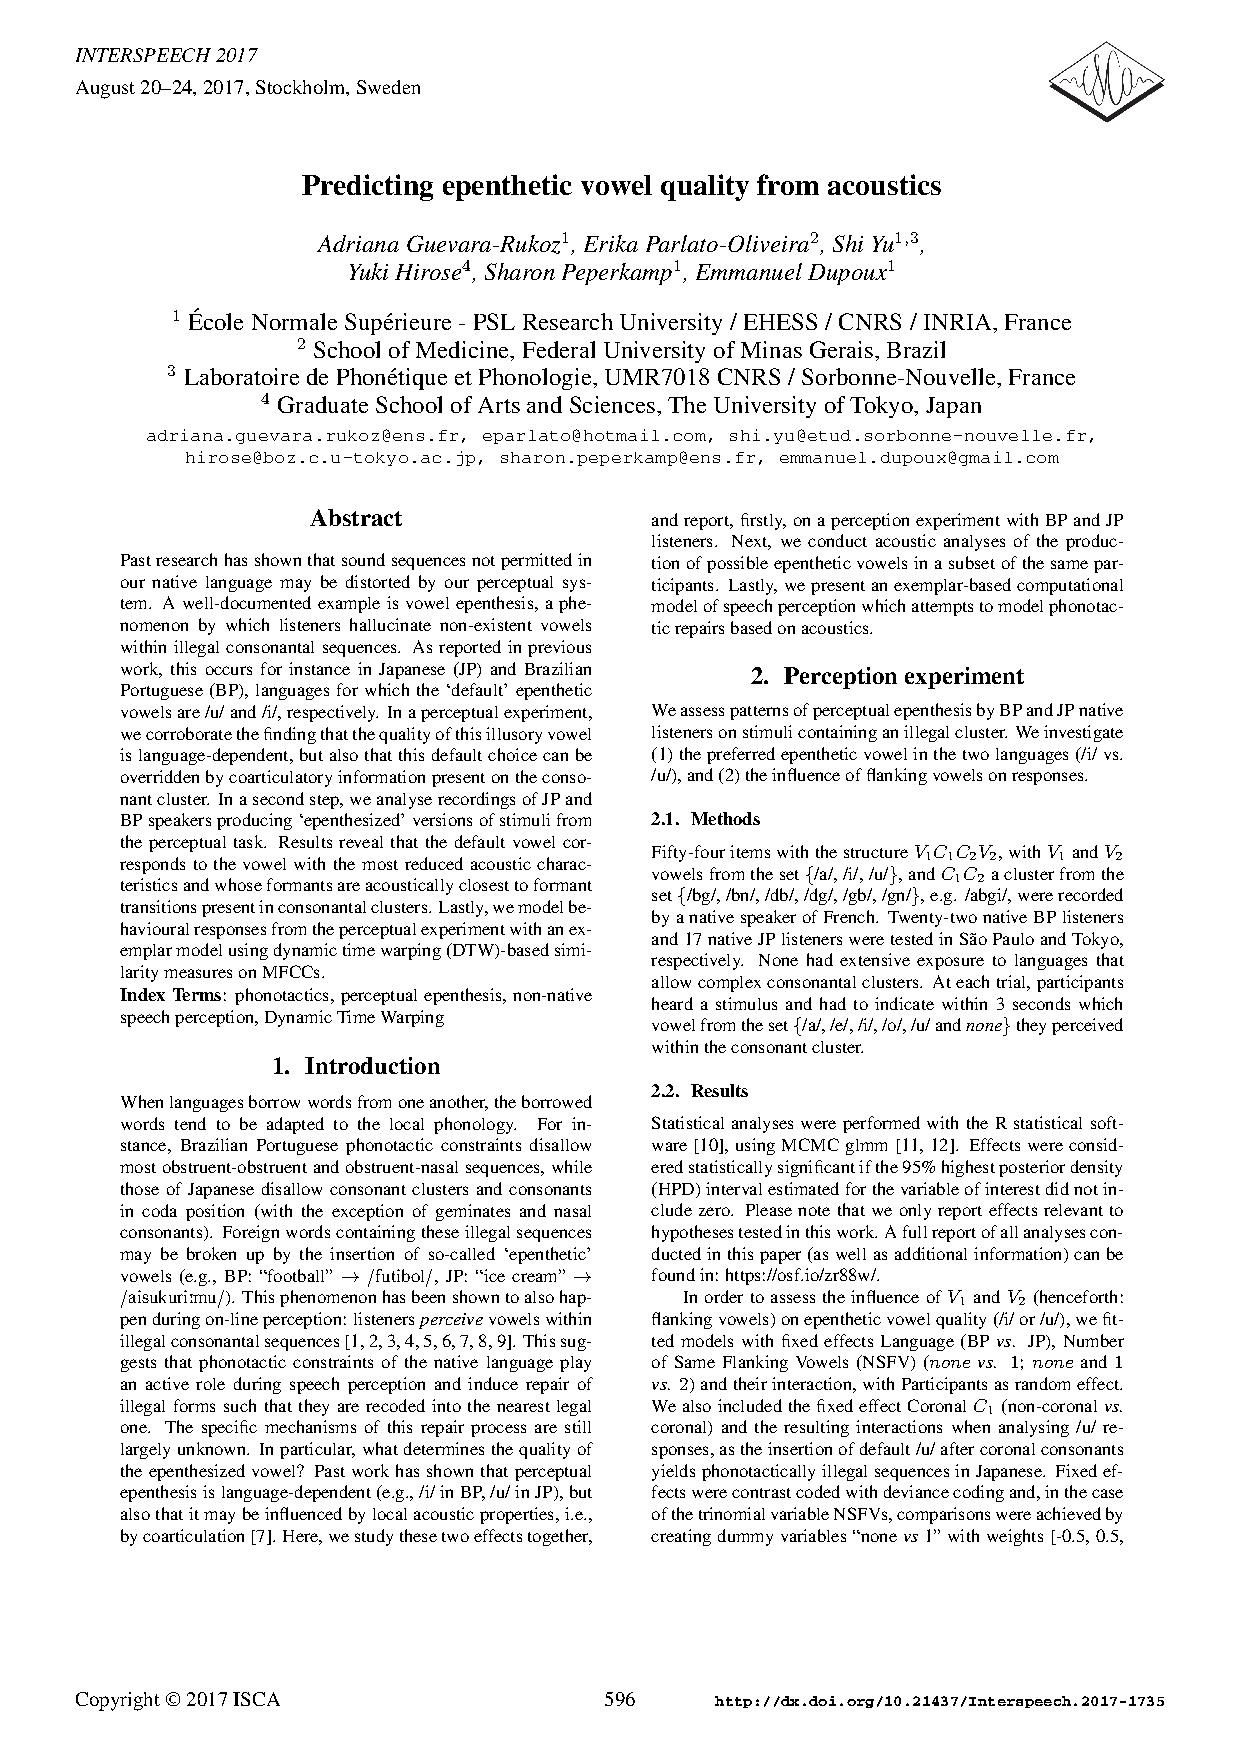
\includepdf[pages={1-5},pagecommand={},
addtotoc={
  1,section,1,Predicting epenthetic vowel quality from acoustics,parlato1_main,
  1,subsection,2,Perception experiment,parlato1_per,
  2,subsection,2,Acoustic analyses,parlato1_prod,
  3,subsection,2,Production-based exemplar model,parlato1_mod,
  4,subsection,2,Discussion,parlato1_disc,
  5,subsection,2,References,parlato1_ref
}]
{images/chapter02/Interspeech2017_Predicting_epenthetic_vowel_quality_from_acoustics_final.pdf}

%%%% Annexes %%%%
\subsection{Annexes}

\subsubsection{Human responses at identification task} 
\begin{figure}[H]
  \centering
  \begin{overpic}[page=1, width=0.6\linewidth]{chapter02/parlato_per_all}\end{overpic}
  \begin{overpic}[page=2, width=0.6\linewidth]{chapter02/parlato_per_all}\end{overpic}
  \caption{Responses from the perception experiment for both BP (top) and JP (bottom), including trials with responses not given by the exemplar model (``none'', ``a'', ``e''). Numbers indicate trial counts, with darker cell backgrounds representing higher values. Within each of the two 3 x 3 grid, trials are separated according to $V_{1}$ (columns) and $V_{2}$ (rows). % [TODO] Check that this is the case and not the other way around 
    Within each individual rectangle, the horizontal axis shows the first consonant of the consonant cluster, while the vertical axis corresponds to possible responses.}
  \label{fig:parlato_per_all}
\end{figure}

\subsubsection{/i/-epenthesis} 
\begin{figure}[h!]
  \centering
  \begin{overpic}[page=1, width=0.45\linewidth]{chapter02/parlato_per_iou}\end{overpic}
  \hspace{1cm}
  \begin{overpic}[page=3, width=0.45\linewidth]{chapter02/parlato_per_iou}\end{overpic}
  \caption{Proportion of /i/-epenthesis in the perception experiment with BP and JP participants (left) and the simulations with the corresponding exemplar-based models (right). Bigger dots show mean values, while smaller dots show individual values for human participants.}
  \label{fig:parlato_uepenth}
\end{figure}

\subsubsection{/u/-epenthesis} 
\begin{figure}[h!]
  \centering
  \begin{overpic}[page=2, width=0.45\linewidth]{chapter02/parlato_per_iou}\end{overpic}
  \hspace{1cm}
  \begin{overpic}[page=4, width=0.45\linewidth]{chapter02/parlato_per_iou}\end{overpic}
  \caption{Proportion of /u/-epenthesis in the perception experiment with BP and JP participants (left) and the simulations with the corresponding exemplar-based models (right). Bigger dots show mean values, while smaller dots show individual values for human participants.}
  \label{fig:parlato_uepenth}
\end{figure}

\subsubsection{Acoustic analyses} 
\begin{figure}[H]
  \centering
  \begin{overpic}[clip, trim=0 0 0 0, page=1, height=6.5cm]{chapter02/parlato_acoustic}\end{overpic}
  \hspace{0.5cm}
  \begin{overpic}[clip, trim=0 0 0 0, page=2, height=6.5cm]{chapter02/parlato_acoustic}\end{overpic}
  \begin{overpic}[clip, trim=0 0 0 0, page=3, height=6.5cm]{chapter02/parlato_acoustic}\end{overpic}
  \caption{Acoustic properties of medial vowels /i, o, u/ produced by BP and JP participants. Distribution of log'd vowel duration (in s), median intensity (in dB) and square root Euclidean distance to template in F1 x F2 x F3 space (frequencies in Bark). Dashed lines show mean values.}
  \label{fig:parlato_prod}
\end{figure}


%%%%%%%%%%%%%%%%%%%%%%%%%%%
% Chapter mini-discussion %
%%%%%%%%%%%%%%%%%%%%%%%%%%%
\section{Summary and Discussion}

%% Summary %%
Summary
\begin{itemize}
\item When coart and flanking V in agreement, predominantly default epV when epenthesis happens (/i/ in BP, /u/ in JP)  
\item Higher influence of acoustic details [coarticulation] on epV quality (section 2.1), reflected by ability of exemplar model to reproduce modulation of epVqual by JP/BP speakers (section 2.2) 
\item Pure acoustic matching not enough (or at least not with current implementation from 2.2); unable to capture striking difference in default epV (+. Role of phonology? (also cf in section 2.1 non-null influence of flanking vowel)
\item 
\end{itemize}


%% Short discussion %%
Model as POC/starting point

\begin{itemize}
\item Lack of duration info because of DTW
\item Assumes exemplar representations
\item Match from acoustics-to-acoustics, without normalizing the acoustics by speaker
\item Inability to model lack of epenthesis -> Yet we see in both sections 2.1 and 2.2 that a significant percentage of responses are ``none''
\end{itemize}

%% Limitations / Remaining questions %%
Going further from epVqual 

\begin{itemize}
\item Focus on effect of acoustics on quality; not denying role of phonology (e.g., phonotactics) on misperception of nonnative clusters 
\item Our results (+ Dup2011) match one-step better than two-step => implementation with more complex one-step model (e.g., HMM using ASR tools)
%\item 
\end{itemize}


%% Conclusion %%
